\section{Netzarchitektur}
\label{raeumliche_netzarchitektur}

Der räumliche Faltungsoperator bildet die erste Faltungsschicht eines neuronalen Netzes auf Graphen~\cite{patchy}.
Dabei kann auf dem berechneten dreidimensionale Tensor der Größe $\left|\gls{V}_{\mathrm{out}}\right| \times \left|\gls{Neighbor}_{\mathrm{out}}\right| \times M$ des Graphen, der zu jeder Knotenauswahl dessen Nachbarschaftsmenge auf dessen $M$ Mermale der Merkmalsmatrix $\gls{F} \in \gls{R}^{N \times M}$ abbildet, mit Hilfe der klassischen Faltungsoperation \gls{conv2d} gefaltet werden (\vgl{}~Abbildung~\ref{fig:netzarchitektur_raeumlich}).
Es ist jedoch insbesondere darauf zu achten, nicht über den Grenzen des Receptive-Fields hinaus zu falten.
Insbesondere sollte eine Faltung entlang der Knotenauswahl $\gls{V}_{\mathrm{out}}$ vermieden werden, da dessen Knotenanordnung im Kontext einer Faltung keine Bedeutung besitzt, denn zwei \enquote{übereinanderliegende} Receptive-Fields müssen nicht zwangsläufig im Graphen benachbart sein.
Die \gls{conv2d}-Operation operiert daher mit der Filtergröße und Schrittweite $1 \times \left|\gls{Neighbor}_{\mathrm{out}}\right|$~\cite{patchy}.
Die restliche Struktur des Netzes kann nach Belieben gewählt werden~\cite{patchy}.
Üblicherweise wird der Ausgabetensor der Faltungsschicht dafür zu einem Vektor umsortiert, sodass vollverbundenen Schichten hin zur Ausgabe an das Ergebnis der Faltungsschicht gestapelt werden können.
Abbildung~\ref{fig:netzarchitektur_raeumlich} veranschaulicht die typische räumliche Netzarchitektur auf Graphen.
\begin{figure}[t]
\centering
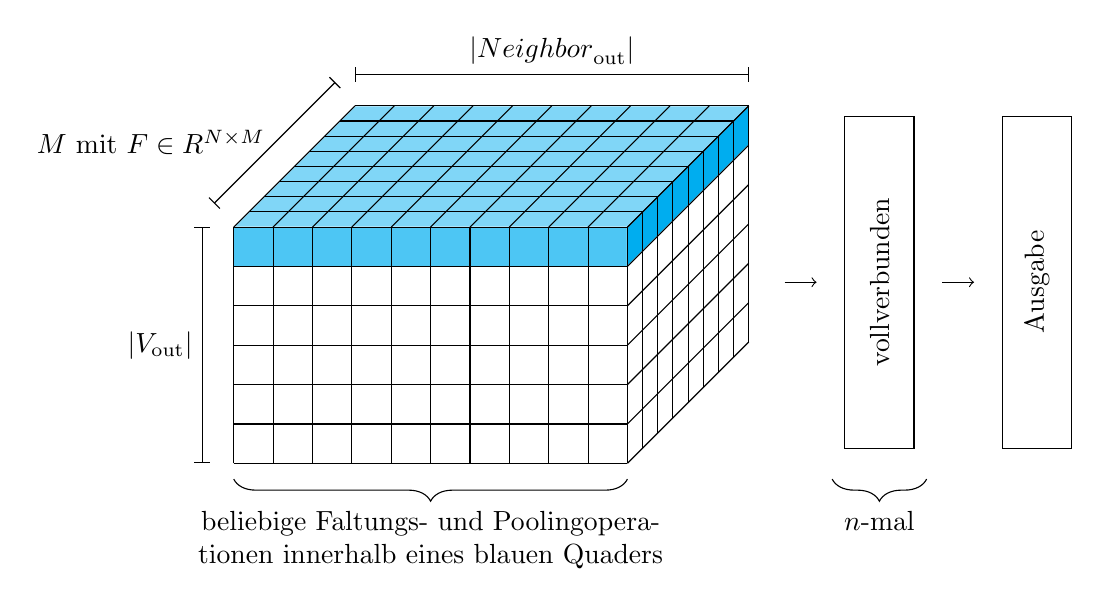
\begin{tikzpicture}
  \draw[white,fill=cyan!70] (0, 3, 4) -- (5, 3, 4) -- (5, 2.5, 4) -- (0, 2.5, 4) -- cycle;
  \draw[white,fill=cyan!50] (0, 3, 4) -- (5, 3, 4) -- (5, 3,   0) -- (0, 3,   0) -- cycle;
  \draw[white,fill=cyan]    (5, 3, 4) -- (5, 3, 0) -- (5, 2.5, 0) -- (5, 2.5, 4) -- cycle;
  \tikzstyle{path}=[->, shorten >= 10pt, shorten <= 10pt]
  \tikzstyle{node}=[rectangle,draw, minimum width=120pt, minimum height=25pt, inner sep=0pt, fill=white, rotate=90]
  \tikzstyle{noborder}=[draw=none,fill=none]

  \foreach \x in {0,0.5,1,1.5,2,2.5,3} {%
    \draw (0,  \x, 4)  -- (5,  \x, 4);
    \draw (5,  \x, 4)  -- (5,  \x, 0);
  }
  \foreach \x in {0,0.5,1,1.5,2,2.5,3,3.5,4,4.5,5} {%
    \draw (\x, 0,  4)  -- (\x, 3,  4);
    \draw (\x, 3,  4)  -- (\x, 3,  0);
  }
  \foreach \x in {0,0.5,1,1.5,2,2.5,3,3.5,4} {%
    \draw (5,  0,  \x) -- (5,  3, \x);
    \draw (0,  3,  \x) -- (5,  3, \x);
  }

  \draw[|-|] (-0.4, 0,    4)    -- node[left]  {$\left|\gls{V}_{\mathrm{out}}\right|$}        (-0.4, 3,    4);
  \draw[|-|] (0,    3.55, 4.65) -- node[left]  {$M$ mit $\ma{F} \in \gls{R}^{N \times M}$}    (0,    3.55, 0.65);
  \draw[|-|] (0,    3.4,  0)    -- node[above] {$\left|\gls{Neighbor}_{\mathrm{out}}\right|$} (5,    3.4,  0);

  \node[node, noborder] (0) at (6.2,  2.3, 4) {};
  \node[node]           (1) at (8.2,  2.3, 4) {vollverbunden};
  \node[node]           (2) at (10.2, 2.3, 4) {Ausgabe};

  \path[path] (0) edge (1);
  \path[path] (1) edge (2);

  \draw [decoration={brace,mirror,amplitude=8pt},decorate,-] (0,-0.2,4) -- node[below=8pt,text width=8cm, align=center] {beliebige Faltungs- und Poolingoperationen innerhalb eines blauen Quaders} (5,-0.2,4);
  \draw [decoration={brace,mirror,amplitude=8pt},decorate,-] (7.6,-0.2,4) -- node[below=8pt] {$n$-mal} (8.8,-0.2,4);

\end{tikzpicture}
\caption[Räumliche Netzarchitektur auf Graphen]{Typische räumliche Netzarchitektur auf Graphen.
Der \emph{Quader}, der durch die Anordnung der Knoten entsprechend ihrer Nachbarschaften entsteht, kann entlang der Nachbarschaften und ihrer Merkmale beliebig oft gefaltet und gepoolt werden.
Eine Faltung entlang der Knotenauswahl besitzt allerdings keine Bedeutung und ist deshalb zu vermeiden.
Im Anschluss können vollverbundene Schichten hin zur Ausgabe an den abgeflachten Quader gestapelt werden.}
\label{fig:netzarchitektur_raeumlich}
\end{figure}


Es ist weiterhin vorstellbar, auch mehrmals in einem Receptive-Field auf analoge Weise zu dem \emph{Fire Module} des \emph{SqueezeNet} zu falten (\vgl{}~\cite{squeeze}).
So können \zB{} über eine Faltung mit Filtergröße und Schrittweite $1 \times 1$ zuvor neue Merkmale aus den Eingabedaten generiert werden und im Anschluss die beschriebene Faltung über das gesamte Receptive-Field vollzogen werden.

Die räumliche Netzarchitektur erlaubt aufgrund ihrer Architektur nur eine Faltungsschicht in einem neuronalen Netz.
Damit sind insbesondere die für das Deep-Learning typischen gestapelten Faltungen mit Poolingoperationen nicht möglich.
Der Ansatz des spektralen Lernens auf Graphen, welcher in Kapitel~\ref{spektrales_lernen} vorgestellt wird, überwindet dieses Problem.
